\documentclass[a0,portrait]{a0poster}
\usepackage[utf8]{inputenc}
\usepackage[T1]{fontenc}
\usepackage{multicol}
\usepackage{graphicx}
\usepackage{amsmath,amsfonts,amssymb}
\usepackage{url}
\usepackage{xcolor}
\usepackage{tikz}
\usepackage{tcolorbox}
\usepackage{enumitem}
\usepackage{booktabs}
\usepackage{caption}
\usepackage{lmodern} % For better font scaling
\usepackage{setspace}
\linespread{1.2} % Adjust line spacing for readability

% Color scheme
\definecolor{tuberlinblue}{RGB}{0,51,102}
\definecolor{tuberlingreen}{RGB}{132,184,24}
\definecolor{lightblue}{RGB}{173,216,230}
\definecolor{darkgray}{RGB}{64,64,64}
\definecolor{lightgray}{RGB}{235,235,235}

% Custom box styles
\tcbset{
    mainbox/.style={
        colframe=tuberlinblue,
        colback=lightgray,
        boxrule=3pt,
        arc=1mm,
        left=5mm,
        right=5mm,
        top=5mm,
        bottom=10mm,
        height=33cm,
    },
    bottombox/.style={
        colframe=tuberlinblue,
        colback=lightgray,
        boxrule=3pt,
        arc=1mm,
        left=5mm,
        right=5mm,
        top=5mm,
        bottom=10mm
    },
    techbox/.style={
        colframe=tuberlingreen,
        colback=white,
        boxrule=1.5pt,
        arc=2mm,
        left=3mm,
        right=3mm,
        top=2mm,
        bottom=2mm
    }
}

\begin{document}
\null  % Provides anchor point for vfill
\vfill

% Header
\begin{center}
	{\VeryHuge\color{tuberlinblue}\textbf{MaRESS: Mapping Research in \\ Earth System Sciences}}\\[1.5cm]
	{\Large\color{darkgray}\textbf{A Modular Web Application for Literature Analysis and Geographic Data Mapping in Earth System Scienes}}\\[0.8cm]

	{\large\color{tuberlinblue}
	\textbf{Benjamin Schmidt}$^1$, \textbf{Marco Otto}$^1$\\[0.3cm]
	$^1$Chair of Climatology, Institute of Ecology, Technische Universität Berlin\\
	Rothenburgstraße 12, 12165 Berlin, Germany\\[0.3cm]
	\texttt{benjamin.schmidt@tu-berlin.de, marco.otto@tu-berlin.de}
	}
\end{center}

\vspace{0.5cm}

% Main content in three columns
\begin{multicols}{3}

	% Column 1: Introduction and Objectives
	\begin{tcolorbox}[mainbox, title={\Large\textbf{Project Overview}}]
		\vspace{0.5cm}
		In the process of conducting systematic literature reviews in Earth System Sciences, researchers often face challenges
		in efficiently geolocating study sites. While study sites are frequently mentioned in the text, they are rarely included
		in machine-readable formats or metadata. This gap hinders the ability to perform comprehensive spatial analyses and
		identify research trends.\\
		\\
		\textbf{MaRESS} (Mapping Research in Earth System Sciences) is a modular web application designed to address these critical challenges in Earth System Sciences research data management and analysis.

		\vspace{0.3cm}
		\textbf{Core Objectives:}
		\begin{itemize}[leftmargin=*]
			\item Automated extraction and mapping of research data from scientific literature
			\item Identification of geographic knowledge voids, thematic research gaps and citation network
			\item Extension of bibliographic metadata with spatial analysis capabilities
			\item AI-assisted categorization and semantic mapping of scientific publications
		\end{itemize}

		\vspace{0.3cm}
		\textbf{Target Application:} Initial deployment will focuses on the expansive test dataset on High Andean Wetlands
		research, supporting comprehensive literature review and ecosystem service analysis
		\vspace{0.5cm}
	\end{tcolorbox}

	\vspace{0.5cm}

	\begin{center}
		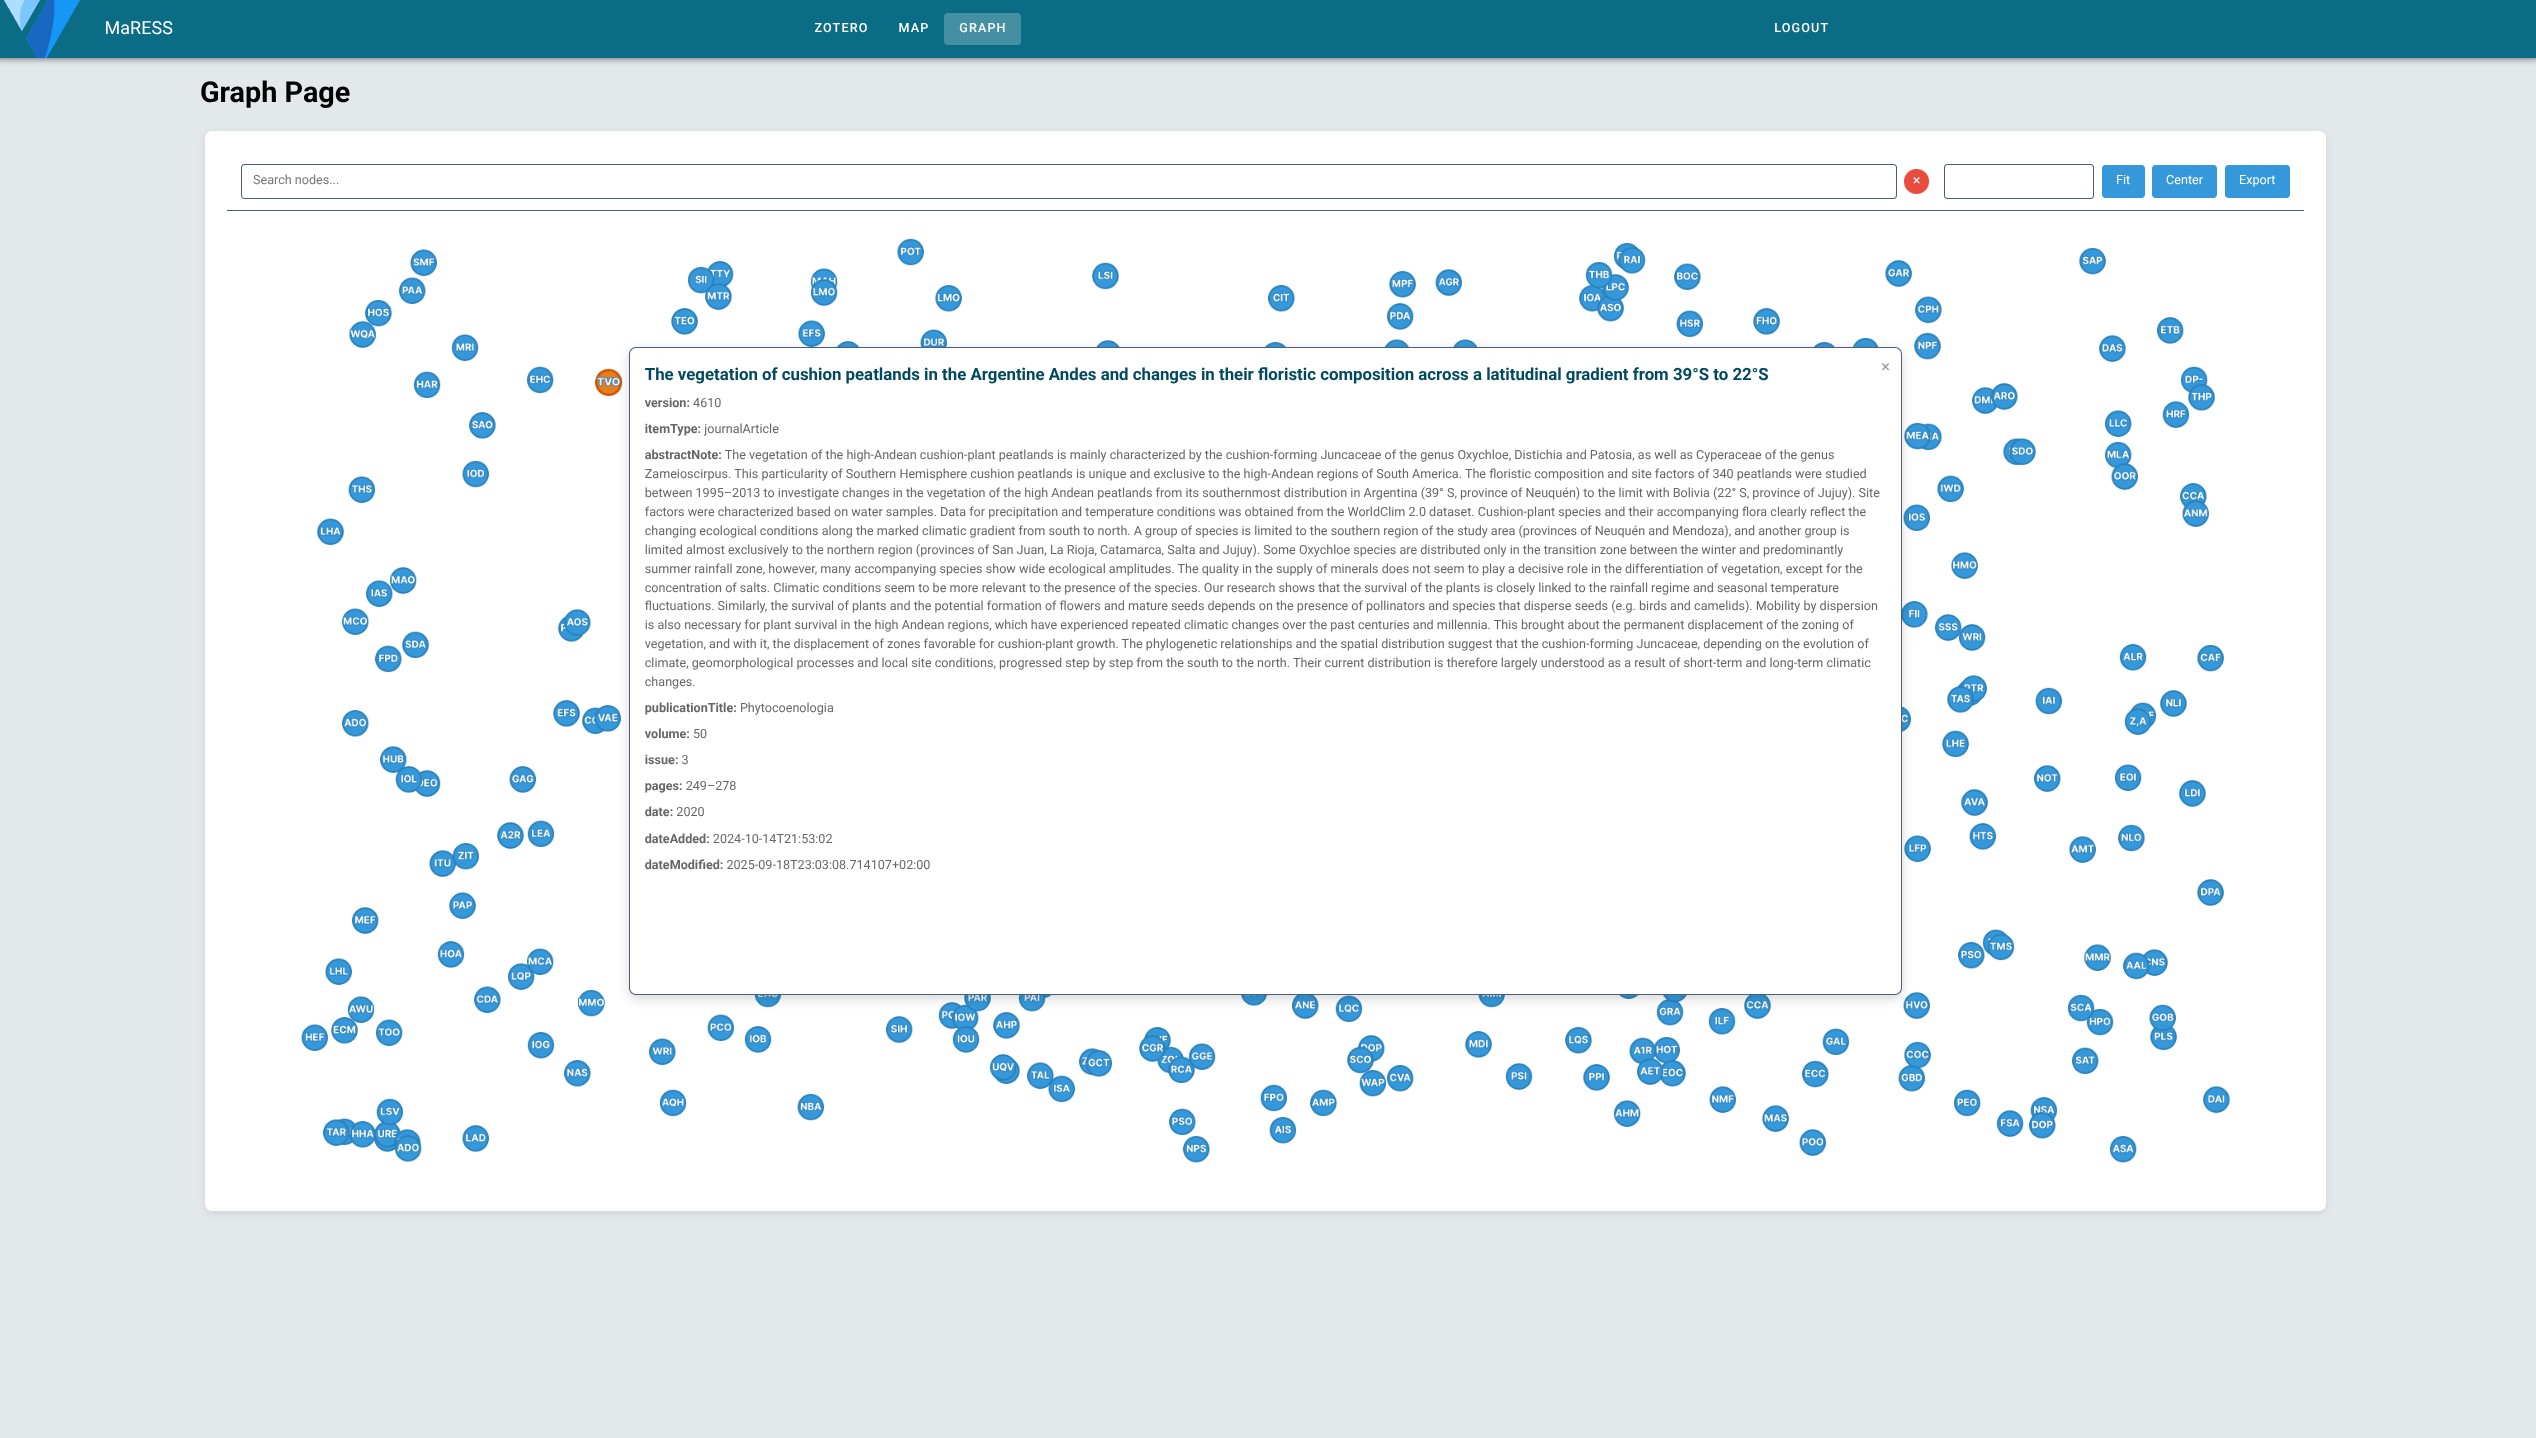
\includegraphics[width=0.9\linewidth]{graph-view}\\
		\vspace{0.2cm}
		{\small Figure 1: \textit{Interactive citation network and keyword visualization using Cytoscape.js with an overlay of metadata
    information of selected paper}}
	\end{center}

	\vspace{0.5cm}

	\begin{tcolorbox}[mainbox, title={\Large\textbf{Technical Architecture}}]
		\vspace{0.5cm}
		\textbf{Backend Infrastructure:}
		\begin{itemize}[leftmargin=*]
			\item Python-based with asynchronous request handling
			\item Relational database with geoinformational extension for spatial data
			\item NLP model pipeline for Named and Custom Entity recognition
			\item Zotero Web API, DataCite DOI resolution, Zenodo integration
		\end{itemize}

		\textbf{Frontend Components:}
		\begin{itemize}[leftmargin=*]
			\item Modern, reactive JS/TS-based Browser application
			\item Interactive geographic visualization with OpenStreetMap and clustering capabilities
			\item Dynamic data tables for metadata filtering and analysis
			\item Cytoscape.js for keyword and author network visualization
		\end{itemize}

		\textbf{Compliance \& Standards:}
		\begin{itemize}[leftmargin=*]
			\item Improves FAIR data principles (Findability, Accessibility)
			\item Open-source licensing (MIT/Apache 2.0)
			\item RESTful API design with OpenAPI 3.1 specification
		\end{itemize}
		\textbf{Deployment:}
		\\Docker containerization ensuring reproducible environments and cross-platform compatibility
		\\ Self{-}hosted or server deployment options
	\end{tcolorbox}

	% Column 2: Methodology and Modules
	\begin{tcolorbox}[mainbox, title={\Large\textbf{Modular System Design}}]
		\vspace{0.5cm}
		\textbf{MaRESS} is structured in frontend/backend architecture, allowing usage as a standalone web application or
		integration into existing research data infrastructures.\\
		Each part is separated technically and functionally into four main modules (Figure 2):

		\vspace{0.5cm}
		\textbf{Module 1: Geographic Mapping}
		\begin{itemize}[leftmargin=*]
			\item Interactive clustered visualization using OpenLayers for Point data
			\item Coordinate extraction from research papers
			\item Spatial clustering analysis of study locations
		\end{itemize}

		\vspace{0.5cm}
		\textbf{Module 2: Semantic Mapping}
		\begin{itemize}[leftmargin=*]
			\item Zotero API integration for bibliographic management
			\item Citation/Author network analysis using graph algorithms
			\item Keyword extraction and clustering
		\end{itemize}

		\vspace{0.5cm}
		\textbf{Module 3: Research Data Mapping}
		\begin{itemize}[leftmargin=*]
			\item Integration with PANGAEA, Zenodo APIs
			\item DataCite DOI metadata extraction
			\item Automated dataset-publication linkage
		\end{itemize}

		\vspace{0.5cm}
		\textbf{Module 4: AI-Assistant}
		\begin{itemize}[leftmargin=*]
			\item Third-party API usage for LLM document categorization
		\end{itemize}
		\vspace{1.3cm}
	\end{tcolorbox}

	\begin{center}
		\vspace{2.2cm}
		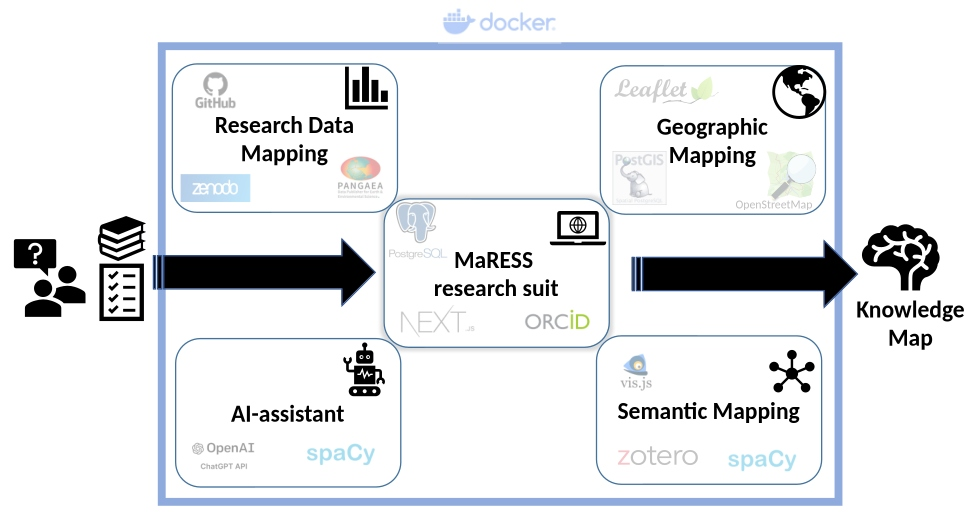
\includegraphics[width=0.9\linewidth]{project-overview}\\
		\vspace{0.2cm}
    {\small Figure 2: \textit{MaRESS modular architecture integrating four core modules}}

		\vspace{3.2cm}
		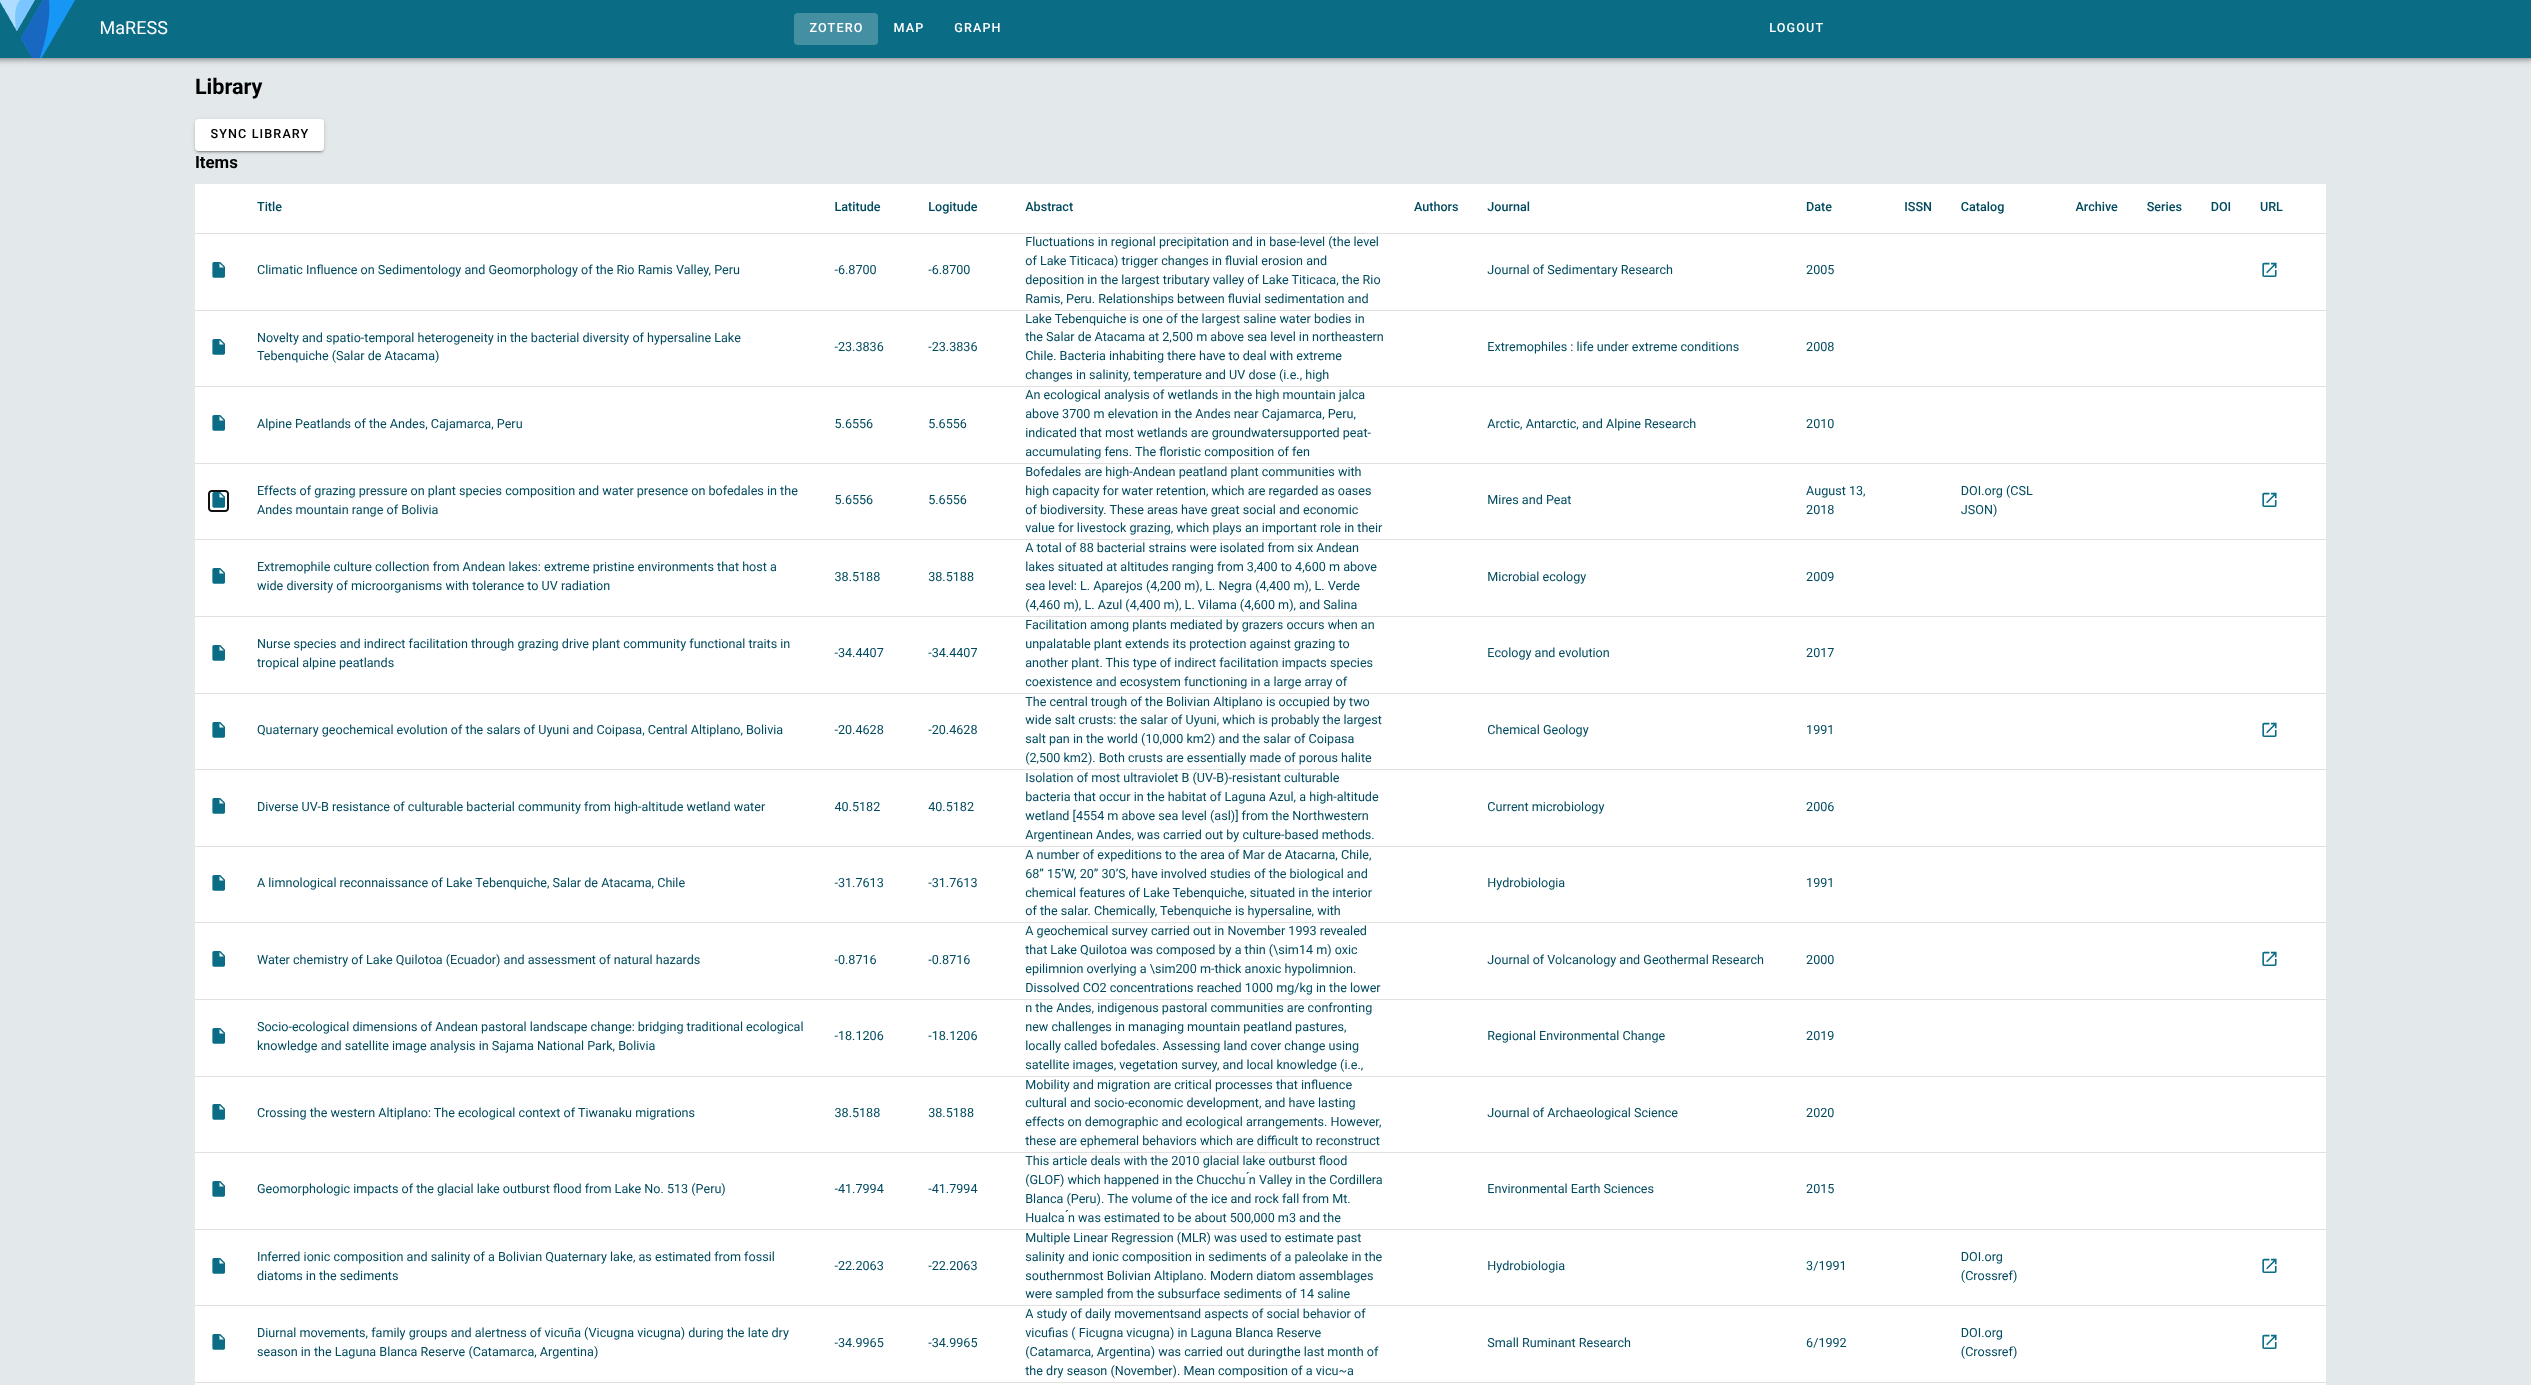
\includegraphics[width=0.9\linewidth]{items-table}\\
		\vspace{0.2cm}
		{\small Figure 3: \textit{Metadata table with sorting, filtering, external links and download options}}
	\end{center}

	\vspace{0.5cm}
	\begin{tcolorbox}[techbox, title={\Large\textbf{Technical Specifications}}]
		\vspace{0.5cm}
		% Using tabular directly without table environment
		\centering
		\begin{tabular}{@{}ll@{}}
			\toprule
			\textbf{Component}           & \textbf{Technology Stack}                        \\
			\midrule
			\textbf{Backend API}         & FastAPI 0.116+ with Pydantic v2                  \\
			\textbf{Database}            & PostgreSQL 17+ with PostGIS 3.3+                 \\
			\textbf{ORM}                 & SQLAlchemy 2.0+ with asyncio support             \\
			\textbf{Authentication}      & OAuth2 + JWT tokens                              \\
			\textbf{NLP Processing}      & spaCy 3.8+ with \texttt{en\_core\_web\_lg} model \\
			\textbf{Frontend Framework}  & Vue.js 3.5+ with TypeScript                      \\
			\textbf{UI Components}       & Vuetify 3.10+ material design                    \\
			\textbf{Mapping Library}     & OpenLayers 10.6+ with vector layers              \\
			\textbf{Graph Visualization} & Cytoscape.js 3.33+                               \\
			\bottomrule
		\end{tabular}
		\vspace{0.5cm}
	\end{tcolorbox}

	\vspace{0.5cm}



	% Column 3: Implementation and Results
	\begin{tcolorbox}[mainbox, title={\Large\textbf{Implementation Workflow}}]
		\vspace{0.5cm}
		\textbf{Data Processing Pipeline:}
		\vspace{0.5cm}
		\begin{enumerate}[leftmargin=*]
			\item \textbf{Authentication:} \\ Current: Email registration with Bearer Token\\ Planned: OAuth2 integration with ORCiD user accounts
			\item \textbf{Metadata Retrieval:} \\ Automated download of bibliographic records and PDFs via \emph{Zotero Web API}
			\item \textbf{NLP Analysis:} spaCy pipeline processes full-text content for:
			      \begin{itemize}
				      \item Geographic entity recognition (GPE, LOC tags)
				      \item Coordinate pattern extraction using regex
				      \item Sentence-level geolocation context analysis
			      \end{itemize}
			\item \textbf{Spatial Analysis:} Algorithms implemented for:
			      \begin{itemize}
				      \item Coordinate validation and projection
				      \item Clustering algorithms (DBSCAN) for study site grouping
			      \end{itemize}
			\item \textbf{Visualization:} Real-time rendering of:
			      \begin{itemize}
				      \item Interactive maps with study location markers
				      \item Citation network graphs with node clustering
				      \item Metadata dashboards with filtering options
			      \end{itemize}
		\end{enumerate}
		\vspace{0.5cm}
	\end{tcolorbox}

	\vspace{0.5cm}

	\begin{center}
		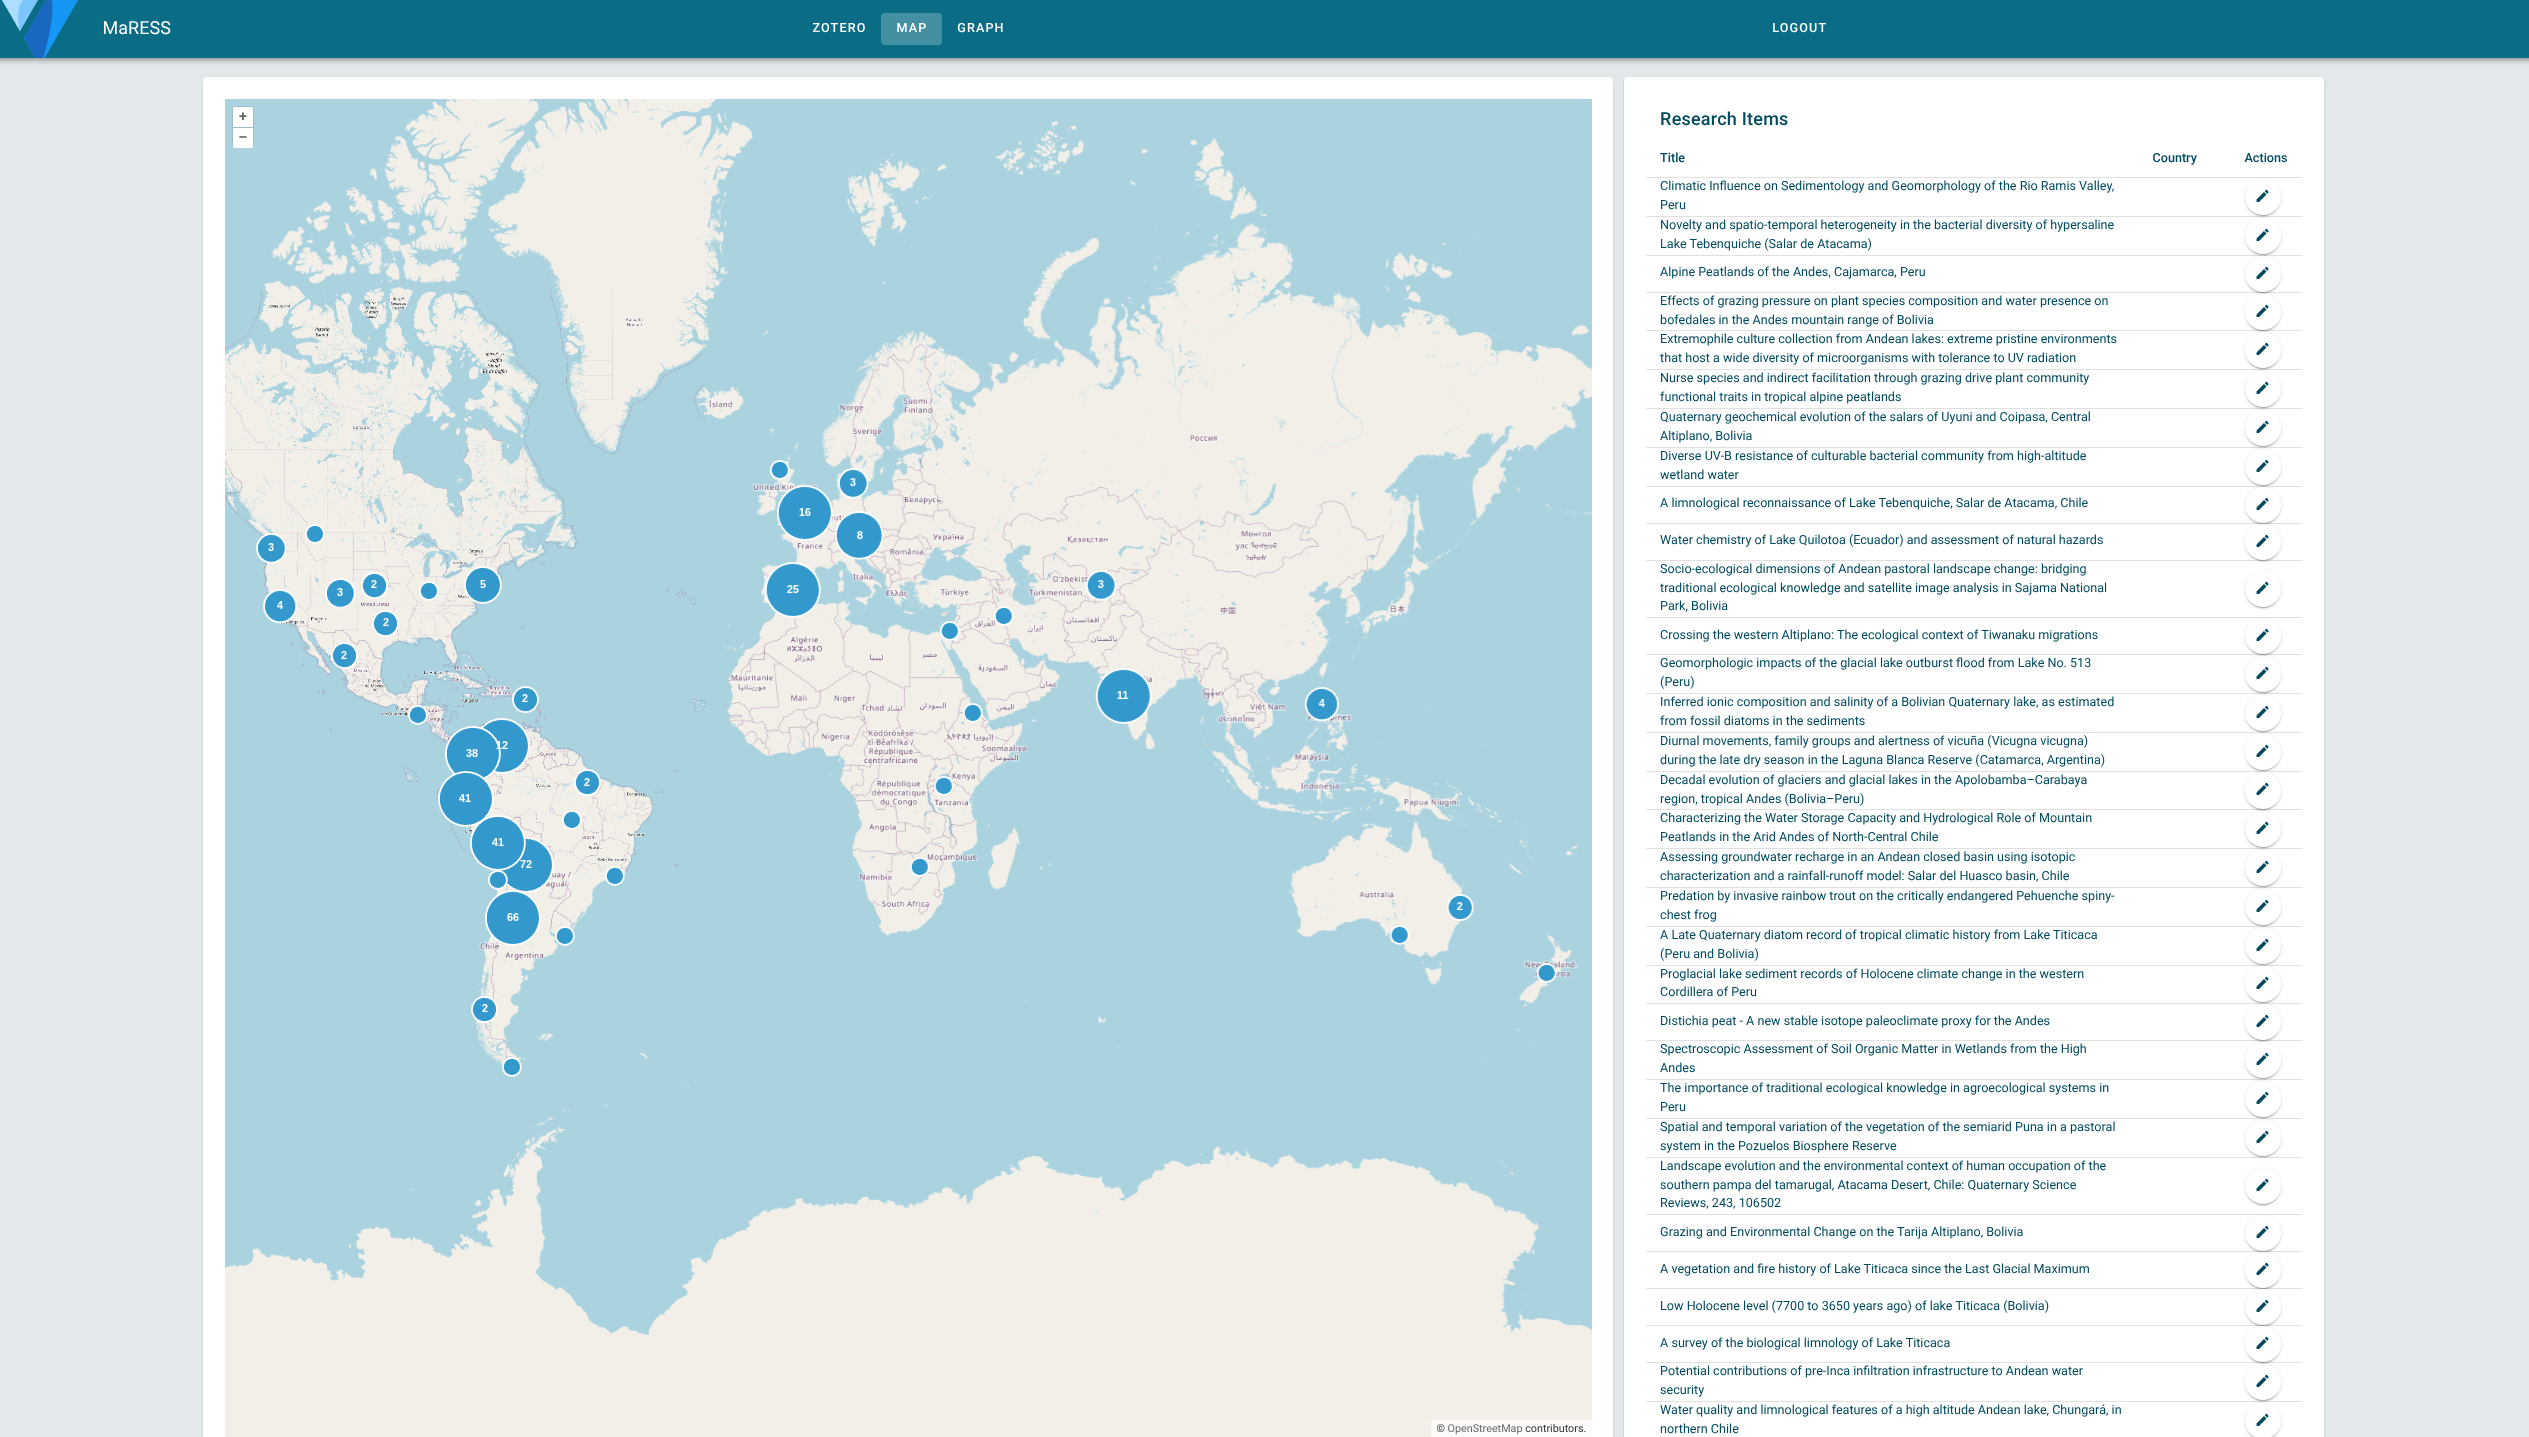
\includegraphics[width=0.9\linewidth]{map-view}\\
		\vspace{0.2cm}
		{\small Figure 4: \textit{Interactive map view displaying clustered research study locations extracted from Zotero
				library via Zotero Web API integration}}
	\end{center}

	\vspace{0.5cm}
	\begin{tcolorbox}[mainbox, title={\Large\textbf{Current Status \& Future Development}}]
		\vspace{0.5cm}
		\textbf{Development Timeline:}
		\begin{itemize}[leftmargin=*]
			\item \textbf{July-September:}
			      \\MaRESS research suite development with User handling
			      \\Zotero API integration for metadata retrieval
			      \\Module 1 (Geographic Mapping) development
			      \\Module 2 (Semantic Mapping) development

			\item \textbf{October:}
			      \\Algorithm accuracy evaluation and improvements
			      \\Missing feature implementation for Modules 1{-}2
			      \\ Implementation of Module 3 (Research Data Mapping)
			\item \textbf{November-December:}
			      \\Final testing and bug fixing
			      \\Module 4 (AI-Assistant) implementation
		\end{itemize}

		\textbf{Key Features Implemented:}
		\begin{itemize}[leftmargin=*]
      \item User authentication and management system
			\item PostgreSQL spatial database with coordinate storage
			\item Automated PDF data processing pipeline (Implementation Workflow)
			\item Cytoscape graph visualization (Figure 1)
      \item Interactive clustered map visualization (Figure 4)
      \item Metadata table with filtering and export options (Figure 3)
		\end{itemize}

	\end{tcolorbox}

\end{multicols}

% Footer
\vspace{0.5cm}
\begin{center}
	\begin{tcolorbox}[bottombox, width=0.9\textwidth]
		\begin{center}
			\textbf{\large Acknowledgments:} This project is supported by NFDI4Earth and carried out at the Chair of Climatology at Technische Universität Berlin. Development infrastructure provided by TU Berlin's Institute of Ecology. Source code will be made available under open-source licensing upon project completion.

			\vspace{0.3cm}
			\textbf{\large Contact:} \url{https://www.tu.berlin/klima} $\bullet$ \url{https://gitlab.klima.tu-berlin.de/klima/maress}
		\end{center}
	\end{tcolorbox}
\end{center}

\vfill
\end{document}

